\textbf{TODO: Summary by Anton}
%%% Local Variables:
%%% mode: latex
%%% TeX-master: "../../report"
%%% End:
\begin{figure}[h]
    \centering
    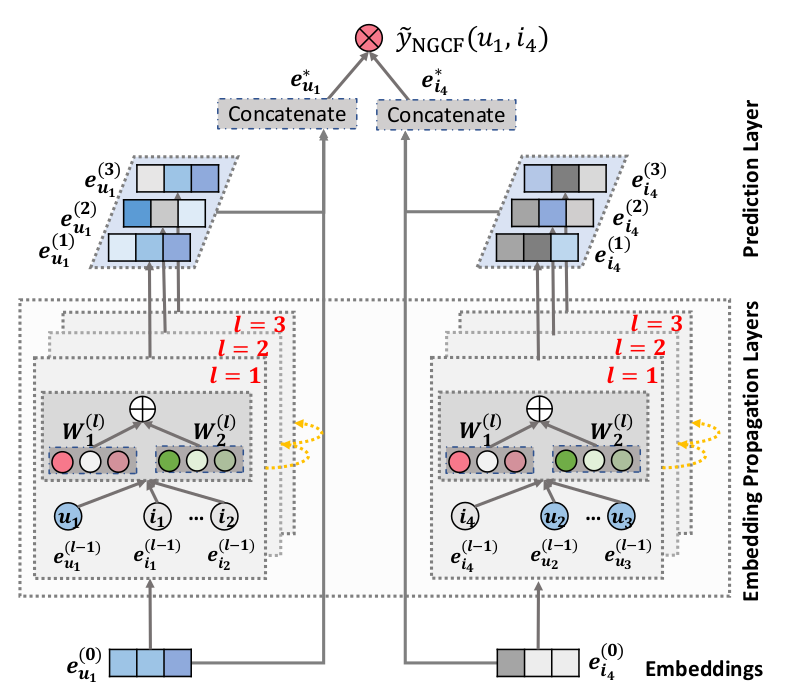
\includegraphics[width=0.8\linewidth]{images/ngcf.png}
    \caption{NGCF architecture.}
    \label{fig:ngcf}
\end{figure}

Tha main difference of NGCF from NCF are the embedding propagation layers which are 
designed to incorporate collaborative signal (especially high-order connectivities 
in users-items connections graph) into embeddings \ref{fig:ngcf}. Therefore, this is supposed to
improve the quality of recommendations.
